\chapterimage{./Pictures/cover-pipe}
\chapter{TP1: Installation et découverte}

\section{Installation et prise en main}
\subsection{Installation du système}
À l'aide de notre live USB nous avons pu installer sur notre HDD externe la distribution de linux appelé "Ubunutu".

\subsection{Découverte du système}
Afin d'accéder à des programmes spécifique ou encore lire et moidifier des fichier system nous avons besoin de la commande \mintinline{shell}{sudo} signifiant \texttt{Super User Do}.

\subsection{Installation des outils nécessaires}
Afin d'avoir les outils des base installer sur la machine nous installons les outils nécessaires à l'aide de la commande \mintinline{shell}{sudo apt install wireshark ethtool iperf openssh-server}.

\section{Découverte de l'environnement}
\subsection{L'interface réseau}
À l'aide de la commande \mintinline{shell}{ifconfig -a} nous pouvons analyser les différentes interfaces réseau.\\
Nous pouvons voir que l'interface appelé \textit{eth0}, n'éxiste plus.

\begin{figure}[H]
\centering
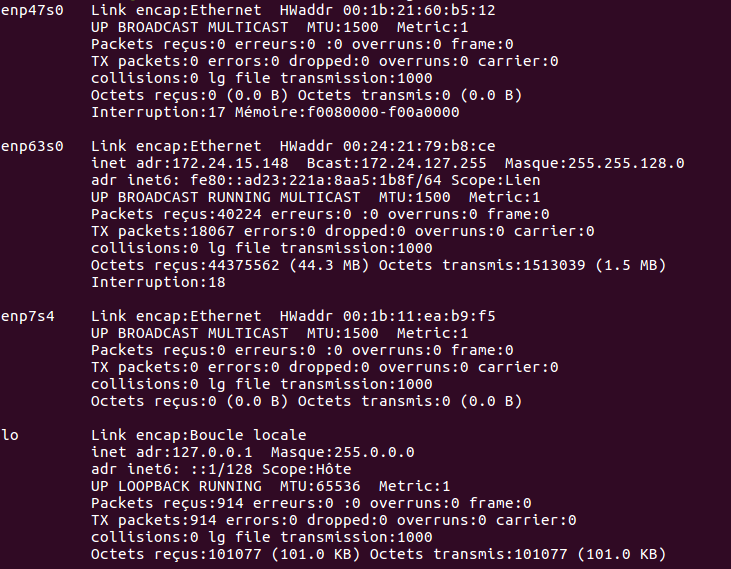
\includegraphics[width=400pt]{./TP1/Pictures/ifconfig}
\caption{Ifconfig}
\label{Ifconfig}
\end{figure}

\begin{itemize}
\item Afin de changer d'address IP nous utiliserons la commande suivante :

\begin{minted}{shell}
ifconfig <INTERFACE> <IP_ADDRESS>
\end{minted}
ainsi la commande \mintinline{shell}{ifconfig enp7s4 198.245.10.0} nous permet de mettre l'address \texttt{198.245.10.0} sur l'interface \texttt{enp7s4}.

\item Afin de changer l'adresse MAC nous utiliserons la commande suivante :
\begin{minted}{shell}
ifconfig <INTERFACE> hw ether <MAC_ADDRESS>
\end{minted}
\item Pour changer l'état d'une interface réseau nous utiliserons la commande :
\begin{minted}{shell}
ifconfig <INTERFACE> [down|up]
\end{minted}
\item Pour afficher l'etat des liens IP nous utiliserons la commande :
\begin{minted}{shell}
ip link show
\end{minted}
\item Pour afficher plus d'informations sur les interfaces réseaux :
\begin{minted}{shell}
ethtool <INTERFACE>
\end{minted}

\end{itemize}

\subsection{État du réseau et connexions actives}
Nous pinguons le site : \texttt{google.fr} à l'aide de la commande :
\begin{minted}{shell}
ping <IP_ADDRESS|URL>
\end{minted}

ainsi la commande \mintinline{shell}{ping google.fr} nous renvoie le texte suivant :
\begin{minted}{shell}
64 bytes from 8.8.8.8: icmp_seq=56 ttl=41 time=19.1 ms
64 bytes from 8.8.8.8: icmp_seq=57 ttl=41 time=19.1 ms
\end{minted}
Nous allons ci-dessous présenter les différents utilisation de la commande \mintinline{shell}{netstat} :
\begin{itemize}
  \item  \mintinline{shell}{netstat} : affiche les connexion réseaux
  \item  \mintinline{shell}{netstat -n} : affiche les adresse au format numerique
  \item  \mintinline{shell}{netstat -a} : affiche tout les socket
  \item  \mintinline{shell}{netstat  --tcp} : définit le protocole à lister (ici TCP)
  \item  \mintinline{shell}{netstat --inet --udp} : définit le protocole a lister (ici udp) aficher selon la methode inet
  \item  \mintinline{shell}{netstat -r --inet -6} : affiche la table de routage selon la methode inet avec ipv6
\end{itemize}

\subsection{La politique de routage}
Afin d'afficher les routes, nous utiliserons la commande \mintinline{shell}{route -n}

\begin{figure}[H]
\centering
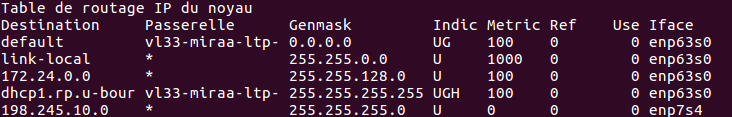
\includegraphics[width=400pt]{./TP1/Pictures/route}
\caption{Route}
\label{Route}
\end{figure}

La ligne 3 correspond au routage du traffic entre les machines de la salle de TP.\\
Une \texttt{passerelle} (\texttt{gateway}) permet d'accéder à un autre réseaux.\\
Si on souhaite envoyer un message à l'adresse 80.80.80.80 on devra utiliser la passerelle par défaut de la ligne 1, via l'interface \texttt{enp63s0}.\\
La passerelle par défaut sur notre machine est la passerelle \texttt{vl33-miraa-ltp-} à l'adresse IP \texttt{172.24.0.1}.

\subsection{Résolution des noms de domaine}
Afin de résoudre un nom domaine, nous utiliserons la commade suivante :
\begin{minted}{shell}
nslookup <URL>
\end{minted}
Ainsi la commande \mintinline{shell}{nslookup www.yahoo.fr} nous renvoie la ŕeponse suivante :
\begin{minted}{bash}
Server:		172.17.0.5
Address:	172.17.0.5#53

Non-authoritative answer:
www.yahoo.fr	canonical name = rc.yahoo.com.
rc.yahoo.com	canonical name = src.g03.yahoodns.net.
Name:	src.g03.yahoodns.net
Address: 212.82.100.150
\end{minted}

Cette réponse venant du serveur DNS à l'adresse IP \texttt{172.17.0.5} nous permet de connaitre l'adresse IP du serveur \texttt{www.yahoo.fr} : 212.82.100.150\\
Le fichier \textit{/etc/resolv.conf} contient les informations de serveur DNS.\\
En ajoutant les correspondance adresse IP <-> nom de domaine au fichier \textit{/etc/hosts} nous pouvons accéder directement aux machines sans passer pas un serveur DNS.

\section{Manipulations avancées}
\subsection{Étude d'une trame ethernet}

Lors de l'utilisation de la commande \mintinline{shell}{ping}, nous observons que la réponse de la commande affiche un champ \textit{TTL}. TTL signifie Time to live, il indique le nombre de saut réstant avant destination. Si le TTL est trop faible, il sera afficher \textit{Time to live exceeded}.\\
À l'aide de Wireshark nous pouvons sniffer le réseau et observer que le protocole utlisé pour la commande \mintinline{shell}{ping} est \textit{ICMP}.
\begin{figure}[H]
\centering
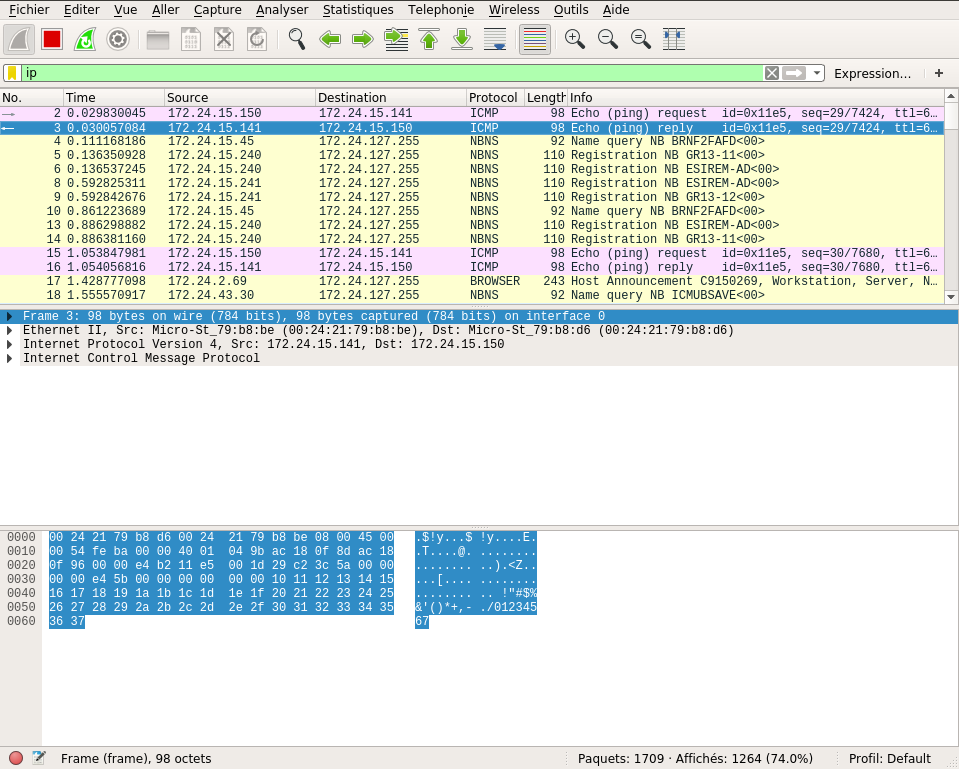
\includegraphics[width=400pt]{./TP1/Pictures/wireshark}
\caption{Wireshark}
\label{Wireshark}
\end{figure}

\subsection{La commande \mintinline{shell}{traceroute}}

La commande \mintinline{shell}{traceroute <IP_ADDRESS>} permet de tracer un paquet depuis un réseau IP vers un hôte donné.\\
En utilisant \mintinline{shell}{traceroute google.fr} nous obtenons la réponse ci-dessous :

\begin{figure}[H]
\centering
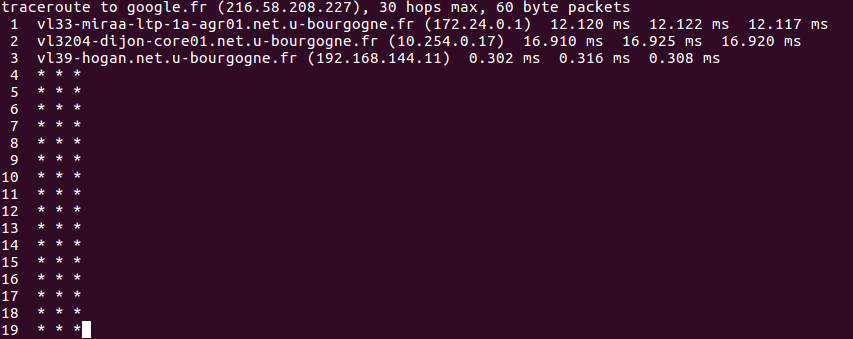
\includegraphics[width=400pt]{./TP1/Pictures/traceroute}
\caption{Traceroute}
\label{Traceroute}
\end{figure}

Les lignes comprenant \texttt{* * *} signifie que le saut sur ce router n'a pas généré de response \texttt{Time-to-live exceeded}\\
On identifie à la première ligne de la réponse l'adresse IP de la passerelle par défaut, ici : \texttt{124.24.0.1}. En effet le premier routeur principale est la passerelle par défaut puisque l'hôte de destination ne fait pas partie du même réseau.
